
\newpage
\customchapter{Simulation results}
\section{Flash instruction memory}

The diagram below demonstrates the procedure of flashing the instruction memory. Throughout this process, the Program Counter (PC) advances by one on each clock cycle, and a byte of data from the hex file, containing instructions, is stored in the byte-addressable instruction memory. Flashing is active only when the flashEn signal is high and the reset signal is low, as indicated in the output. This operation of flashing takes about 290 nanoseconds to write 28 bytes of 7 RISC-V instructions into the instruction memory.

\begin{figure}[h!]
    \centering
    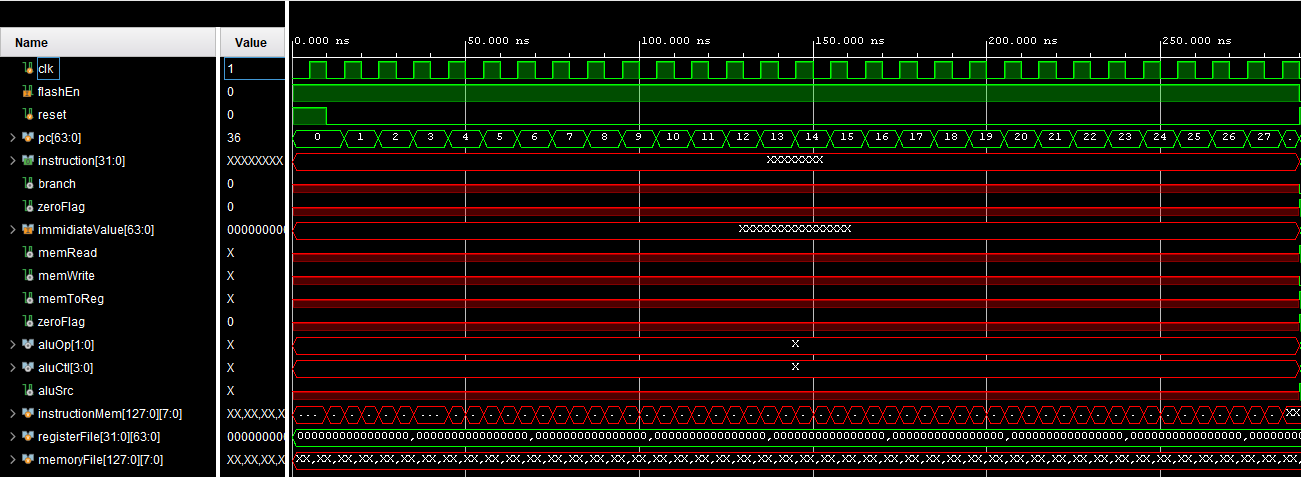
\includegraphics[width=0.9\textwidth, height=0.3\textheight]{Image/01_Sim.png}
    \caption{Instruction Memory Flashing Process}
    \label{fig:flash_memory}
\end{figure}

\section{Processor simulation}

After the instructions have been flashed into memory, the processor can be reset, causing the PC to reset to zero. Subsequently, the processor begins fetching instructions from the memory starting at address zero. This behavior is depicted in the image below. To facilitate explanation, the following timelines are considered:

\begin{figure}[h!]
    \centering
    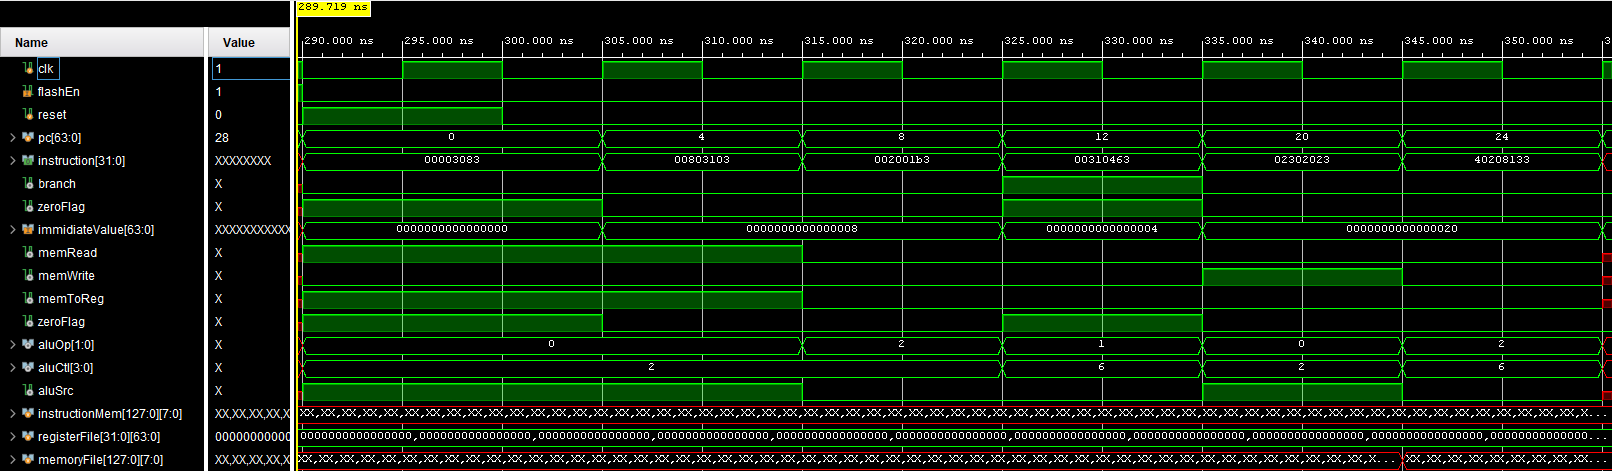
\includegraphics[width=1.0\textwidth, height=0.23\textheight]{Image/02_sim.png}
    \caption{Processor Simulation}
    \label{fig:processor_simulation}
\end{figure}

\begin{itemize}
    \item \textbf{Time Stamp (290ns – 300ns):} The reset signal gets pulsed, the PC becomes zero, and fetches the first instruction \texttt{ld r1 0(r0)} where \texttt{r0=0} with the hex code of \texttt{0x00003083} gets executed which fetches a double word from \texttt{0x00} data memory location into the \texttt{r1} register of the register file.
    \item \textbf{Time Stamp (300ns – 310ns):} Now \texttt{PC=4} and the next instruction gets fetched \texttt{ld r2 8(r0)} where \texttt{r0=0} with the hex code of \texttt{0x00803103} gets executed which fetches a double word from \texttt{0x08} data memory location into the \texttt{r2} register of the register file.
    \item \textbf{Time Stamp (310ns – 320ns):} Now \texttt{PC=8} and the next instruction gets fetched \texttt{add r3 r2 r0} with the hex code of \texttt{0x002001b3} gets executed which adds the data present in \texttt{r0} and \texttt{r2} registers and then stores the result in the \texttt{r3} register.
    \item \textbf{Time Stamp (320ns – 330ns):} Now \texttt{PC=12} and the next instruction gets fetched \texttt{beq r3 r2 4(offset)} with the hex code of \texttt{0x00310463} gets executed which checks if \texttt{r3==r2}, if yes then it gets branched to target address \texttt{(currentPC+4) + 4(offset)}. So \texttt{newPC = 20}. Also, observe imidiateValue during branch.
    \item \textbf{Time Stamp (330ns – 340ns):} Now \texttt{PC=20} and the next instruction gets fetched \texttt{sd r3 32(r0)} with the hex code of \texttt{0x02302023} gets executed which stores data present in \texttt{r3} at \texttt{r0+32}.
    \item \textbf{Time Stamp (340ns – 350ns):} Now \texttt{PC=24} and the next instruction gets fetched \texttt{sub r2 r2 r1} with the hex code of \texttt{0x40208133} gets executed which subtracts \texttt{r2 – r1} and stores back data into \texttt{r2}.
\end{itemize}




